\documentclass[a4paper]{article}
\usepackage[utf8]{inputenc}
\usepackage[slovene]{babel}
\usepackage{graphicx}
\usepackage{hyperref}
\usepackage[nottoc]{tocbibind}
\usepackage{minted}
\usepackage{listings}
\usepackage{caption}
\usepackage{subcaption}
\usepackage{amsmath}
\usepackage{ dsfont }
\usepackage{siunitx}
\usepackage{multimedia}
\usepackage[table,xcdraw]{xcolor}
\setlength\parindent{0pt}

\usepackage{soul}

\definecolor{codegreen}{rgb}{0,0.6,0}
\definecolor{codegray}{rgb}{0.5,0.5,0.5}
\definecolor{codepurple}{rgb}{0.58,0,0.82}
\definecolor{backcolour}{rgb}{0.95,0.95,0.92}
\newcommand{\ddd}{\mathrm{d}}
\newcommand\myworries[1]{\textcolor{red}{#1}}
\newcommand{\Dd}[3][{}]{\frac{\ddd^{#1} #2}{\ddd #3^{#1}}}

\lstdefinestyle{mystyle}{
    backgroundcolor=\color{backcolour},   
    commentstyle=\color{codegreen},
    keywordstyle=\color{magenta},
    numberstyle=\tiny\color{codegray},
    stringstyle=\color{codepurple},
    basicstyle=\ttfamily\footnotesize,
    breakatwhitespace=false,         
    breaklines=true,                 
    captionpos=b,                    
    keepspaces=true,                 
    numbers=left,                    
    numbersep=5pt,                  
    showspaces=false,                
    showstringspaces=false,
    showtabs=false,                  
    tabsize=2
}

\lstset{style=mystyle}

\begin{document}
\begin{titlepage}
    \begin{center}
        
\includegraphics[]{logo.png}
        \vspace*{3cm}
        
        \Huge
        \textbf{Diferenčne metode za parcialne diferencialne enačbe}
        
        \vspace{0.5cm}
        \large
        10. naloga pri Matematično-fizikalnem praktikumu

        \vspace{4.5cm}
        
        \textbf{Avtor:} Marko Urbanč (28191096)\ \\
        \textbf{Predavatelj:} prof. dr. Borut Paul Kerševan\ \\
        
        \vspace{2.8cm}
        
        \large
        4.9.2023
    \end{center}
\end{titlepage}
\tableofcontents
\newpage
\section{Uvod}
V prejšnji nalogi smo rekli, da obstajata v glavnem dva velika razreda za reševanje parcialnih diferencialnih
enačb (PDE). To sta spektralne metode, ki smo jih raziskali v prejšnji nalogi in pa diferencialne metode, ki jih
spoznamo tu. Diferencialne metode so v glavnem metode, ki rešujejo PDE tako, da jih diskretizirajo in jih
pretvorijo v sistem linearnih enačb. Te metode so v glavnem zelo podobne kot metode za reševanje sistemov
navadnih diferencialnih enačb (ODE). V glavnem se razlikujejo v tem, da so PDE lahko tudi nelinearne in
moramo posledično uporabiti iterativne metode za reševanje sistemov linearnih enačb. Tu bomo spoznali 
metodo končnih diferenc (FDM). Ta temleji na Taylorjevem razvoju s katerim lahko aproksimiramo odvod
funkcije. To aproksimacijo nato vstavimo v PDE in dobimo sistem linearnih enačb. Ta sistem nato rešimo
iterativno in dobimo končno rešitev. \\

Fizikalni kontekst za to nalogo bo reševanje enodimenzionalne nestacionarne Schrödingerjeve enačbe, ki se
glasi

\begin{equation}
    \left( i\hbar \frac{\partial}{\partial t} - H\right) \psi(x,\>t) = 0\>.
    \label{schrodinger}
\end{equation}

Predstavlja osnovno orodje za nerelativistični opis kvantnih sistemov. V enačbi (\ref{schrodinger}) je $H$ Hamiltonian
sistema, ki je v splošnem odvisen od časa. V našem primeru bomo obravnavali časovno neodvisen Hamiltonian

\begin{equation}
    H = -\frac{\hbar^2}{2m} \frac{\partial^2}{\partial x^2} + V(x)\>.
    \label{hamiltonian}
\end{equation}

Z menjavo spremenljivk $H/\hbar \rightarrow H$, $x\sqrt{m/\hbar} \rightarrow x$ efektivno postavimo $\hbar = m = 1$.
V tem primeru je Hamiltonian enak

\begin{equation}
    H = -\frac{1}{2} \frac{\partial^2}{\partial x^2} + V(x)\>.
    \label{hamiltonian2}
\end{equation}

Razvoj stanja $\psi(x,\>t)$ v času $\psi(x,\>t + \Delta t)$ je opisan z približkom

\begin{equation}
    \psi(x,\>t + \Delta t) = e^{-iH\Delta t}\psi(x,\>t)\approx \dfrac{1-\frac{1}{2}iH\Delta t}
    {1+\frac{1}{2}iH\Delta t}\psi(x,\>t)\>.
    \label{razvoj}
\end{equation}

Območje $x\in[a,\>b]$ diskretiziramo na krajevno mrežo z $N$ točkami $x_j = a + j\Delta x$, kjer je $\Delta x = (b-a)/(N-1)$.
Časovni razvoj spremljamo ob časovni mreži z $M$ točkami $t_m = m\Delta t$, kjer je $\Delta t$ časovni korak. Vrednosti valovne
funkcije in potenciala v mrežnih točkah ob času $t_m$ označimo z $\psi_j^m$ in $V_j$. Krajevni odvod izrazimo z 
diferenco

\begin{equation}
    \Psi''(x) \approx \frac{\psi(x + \Delta x,\>t)-2\psi(x,\>t)+\psi(x-\Delta x,\>t)}{\Delta x^2} 
    = \frac{\psi_{j+1}^m - 2\psi_j^m + \psi_{j-1}^m}{\Delta x^2}\>.
    \label{krajevni_odvod}
\end{equation}

Te približke vstavimo v razvoj stanja (\ref{razvoj}) in razpišemo Hamiltonov operator, da dobimo sistem enačb

\begin{multline}
    \psi_j^{m+1} - i \frac{\Delta t}{4\Delta x^2}\left[\psi_{j+1}^{m+1} - 2\psi_j^{m+1} + \psi_{j-1}^{m+1}\right] + i \frac{\Delta t}{2} V_j \psi_j^{m+1} = \\
    \psi_j^m + i \frac{\Delta t}{4\Delta x^2}\left[\psi_{j+1}^m - 2\psi_j^m + \psi_{j-1}^m\right] - i \frac{\Delta t}{2}V_j\psi_j^m\>.
    \label{sistem}
\end{multline}

v notranjih točkah mreže, medtem ko na robu (pri $j\le 0$ in $j\ge N$) postavimo $\psi_j^{m} = 0$. Vrednosti valovne funkcije uredimo v 
vektor $\Psi^m$ in sistem (\ref{sistem}) prepišemo v matrično obliko

\begin{equation}
    \mathbf{A}\Psi^{m+1} = \mathbf{A^*}\Psi^m\>,
\end{equation}

kjer je $\mathbf{A}$ tridiaonalna matrika z elementi

\begin{equation}
    b = 1 + i\frac{\Delta t}{2\Delta x^2}\>,\quad a = -\frac{b}{2}\>,\quad d_j = 1 + b + i\frac{\Delta t}{2}V_j\>.
\end{equation}
Torej je $\mathbf{A}$ oblike

\begin{equation}
    \mathbf{A} = \begin{bmatrix}
        d_1 & a & 0 & \cdots & 0 \\
        a & d_2 & a & \cdots & 0 \\
        0 & a & d_3 & \cdots & 0 \\
        \vdots & \vdots & \vdots & \ddots & \vdots \\
        0 & 0 & 0 & \cdots & d_{N-1}
    \end{bmatrix}\>.
\end{equation}

Kot smo napovedali, je to torej matrični sistem, ki ga moramo rešiti v vsakem časovnem koraku iterativno.

\section{Naloga}
Naloga je sestavljena iz dveh delov. V prvem delu naloga od nas zahteva, da spremljamo časovni razvoj 
začetnega stanja

\begin{equation}
    \Psi(x,\>0) = \sqrt{\frac{\alpha}{\sqrt{\pi}}} e^{-\alpha^2(x-\lambda)^2/2}\>,
    \label{zacetno_stanje1}
\end{equation}

v harmonskem porencialu $V(x) = 1/2\cdot k x^2$, kjer je $\alpha = k^{1/4}$ in $\omega = \sqrt{k}$.
Analitična rešitev za to stanje je

\begin{equation}
    \psi(x,\>t) = \sqrt{\frac{\alpha}{\sqrt{\pi}}} \exp{\left[-\frac{1}{2}(\xi - 
    \xi_\lambda \cos{\omega t})^2-
    i\left(\frac{\omega t}{2} + \xi\xi_\lambda \sin{\omega t} - 
    \frac{1}{4}\xi_\lambda^2\sin{2\omega t}\right)\right]}\>,
    \label{analiticna_resitev1}
\end{equation}

kjer je $\xi=\alpha x$ in $\xi_\lambda = \alpha\lambda$. Postavimo $\omega=0.2$ in $\lambda=10$.
Za krajevno mrežo vzamemo razpon $x\in[-40, 40]$ in $N=300$ točk. Nihajni čas je $T=2\pi/\omega$,
zato primerno prilagodimo časovni korak $\Delta t$ in stanje opazujemo deset period. V drugem delu naloge pa moramo spremljati razvoj gaussovskega valovnega paketa 

\begin{equation}
    \Psi(x,\>0) = (2\pi\sigma_0^2)^{-1/4} e^{ik_0(x-\lambda)}e^{-(x-\lambda)^2/(2\sigma_0)^2}\>.
    \label{zacetno_stanje2}
\end{equation}

v praznem prostoru $V(x) = 0$. Analitična rešitev za to stanje je

\begin{equation}
    \psi(x,\>t) = \frac{(2\pi\sigma_0^2)^{-1/4}}{\sqrt{1 + i t/(2\sigma_0^2)}}
    \exp{\left[\frac{-(x-\lambda)^2/(2\sigma_0^2) + ik_0(x-\lambda)-ik_0^2 t/2}
    {\sqrt{1 + i t/(2\sigma_0^2)}}\right]}
    \label{analiticna_resitev2}
\end{equation}

Tu vzamemo območje $x\in[-0.5, 1.5]$ in spremljamo dokler paket ne prečka $x\approx 0.75$.
Postavimo $\sigma_0=1/20$, $k_0=50\pi$ in $\lambda=0.25$.

\section{Opis reševanja}
Zdaj praktično delam ``faks zaključek'' speedrun, torej ta naloga žal ni tako podrobno rešena,
kot bi mogoče želel. Uporabil sem standardni ansambel programskih paketov, ki sem jih uporabljal
tudi pri prejšnji nalogi. Torej \texttt{numpy}, \texttt{scipy} in \texttt{matplotlib}. Pri tej nalogi
žal nisem imel možnosti (zaradi omejenega časa), da bi delal kakšne divje eksperimente, torej je to praktično to
kar se tiče programske opreme.\\

\subsection{FDMSolver}
Programersko sem se naloge lotil identično kot pri prejšnji nalogi. Torej sem napisal razred \texttt{FDMSolver},
ki vsebuje vse potrebne metode za reševanje te naloge. V konstruktorju razreda \texttt{FDMSolver} se inicializira
vse potrebno, od tam naprej pa lahko uporabnik kliče razne funkcije. Večina jih je pravzaprav za risanje, saj je 
razred priročen storage za vse potrebne podatke in posledično risarski funkciji ni potrebno podati ogromno argumentov.
V glavnem je razred \texttt{FDMSolver} zelo podoben kot \texttt{SpectralSolver} iz prejšnje naloge. Glavna razlika
in cel point nalog pa je njegova metoda \texttt{solve()}. Tu se incializirajo še potrebne matrike in se začne iterativno
reševanje sistema. Pravzaprav tu tokrat nisem naredil res čisto nič posebnega, samo običajno matrično množenje
\texttt{numpy} \texttt{ndarray}-ov. Se mi zdi škoda, ker bi lahko preverjal svojo implementacijo proti kaki, ki jo 
ima recimo \texttt{scipy} ali pa \texttt{numpy}. Recimo \texttt{scipy.sparse.linalg.bicgstab()} se mi zdi. Ali pa v našem
primeru, ker imamo tridiagonalno matriko bi moral dobro delati \texttt{scipy.linalg.solve\_banded()}. 
Anyways žal tega nisem imel časa narediti.\\

\section{Rezultati}
\subsection{Prvi primer - harmonski oscilator}
Za prvi primer sem uporabil začetno stanje (\ref{zacetno_stanje1}).
Začetno stanje sem diskretiziral na mrežo z $N=300$ točkami, vsaj prvotno. Izkazalo se je,
da pri nastavitvah, ki so predlagane v nalogi, rešitev čez nekaj nihajev razpade. Nedopustno.
Čas sem spremljal originalno na mreži z 
$M=1100$ točkami torej $100$ na periodo, kjer je bilo period potem $11$. To se mi je zdelo sila bedno. 
Plačal sem za cel procesor, uporabljal bom cel procesor. Tako sem časovno mrežo razširil na $M=11000$ točk.
Matrično množenje v \texttt{numpy} je že po defaultu paralelizirano, torej very nice. \\

Zdelo se mi je zanimivo, da bi poiskal okvirno koliko točk potrebjemo za smiselno rešitev (torej, takšno,
ki ne razpade po 10 nihajih). Ugotovil sem, da je spodnja meja okoli $N=200$. Zdaj, če bi imel čas 
bi šel seveda te stvari vse dejansko izvest, ampak zanimivo bi bilo, kolikšen je dejansko performance
gain oz. krajši čas računanja. Ker meni se je zdelo $N = 200,\> M = 11000$ opazno hitrejše kot 
$N = 300,\> M = 1100$. Recimo če zdaj gledamo large scale in si predstavljamo, da rešujemo res nek 
zakompliciran velik model, na porazdeljenem sistemu, se mi zdi zelo koristna metrika, za koliko 
več elektrike (oz. cloud hosting resources) bo potrebno plačati za tistih več točk in
kolikšna bo izboljšava v dobljenem rezultatu. \\

Predstavim recimo lahko tale graf, ki se mi je zdel razmeroma zanimiv (pa zato, ker drugih, niti
nimam). Predstavlja razliko med rešitvijo z zelo gosto mrežo $N=700$ in z našo domnevno spodnjo
mejo $N=200$. Časovni grid je bil v obeh primerih $M=11000$. Vidimo, da je razlika v rešitvi
zelo zelo majhna, do te mere, da me skrbi, da sem kje kaj zamočil in tega nisem pravočasno opazil.
Ampak vizualno, ko človek gleda dobljene animacije zgledata res identično.

\begin{figure}[H]
    \centering
    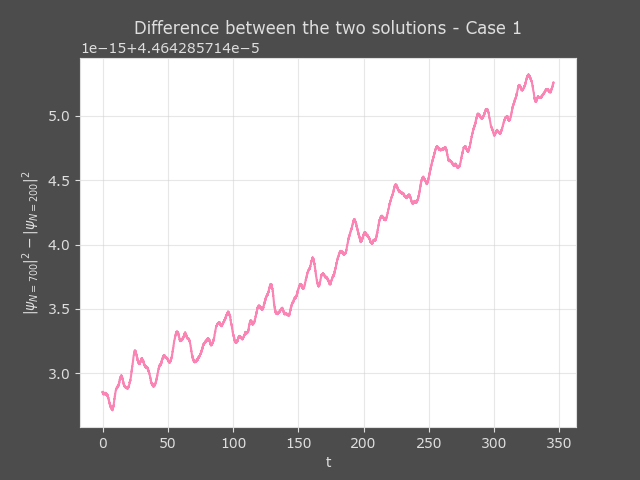
\includegraphics[width=\textwidth]{./images/delta_N700_N200.png}
    \caption{Razlika med rešitvama z $N=700$ in $N=200$}
\end{figure}

Pa ja, razlika med rešitvama definitivno narašča z časom, kot je pričakovano, saj se rešitve še vedno kvarijo
in sklepam, da se tista pri $N=200$ kvari hitreje, ampak bralec, poglej ta red velikosti razlike. \\

Kakorkoli zdaj je dovolj o tem, da sem se igral z različnimi parametri. Glavni obrok je serviran! Na Sliki
\ref{fig:harmonic_oscillator_org} je prikazana rešitev pri originalnih parametrih, torej $N=300$, $M=1100$. \\

\subsubsection{Komentarji k glavnemu obroku}

\begin{figure}[p]
    \centering
    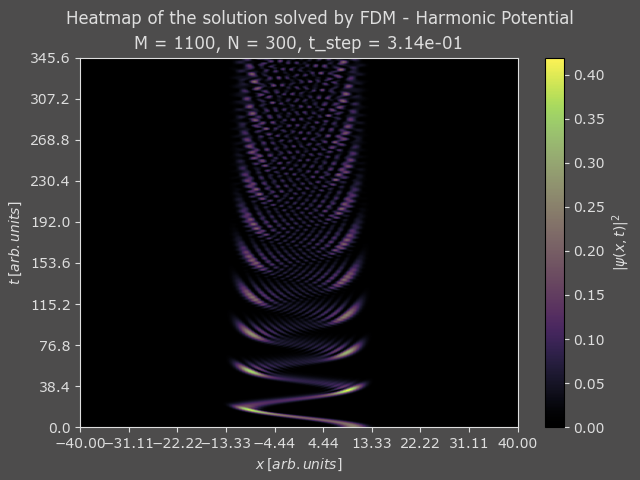
\includegraphics[width=\textwidth]{./images/case1_org.png}
    \caption{Rešitev pri originalnih parametrih.}
    \label{fig:harmonic_oscillator_org}
\end{figure}

Na Sliki \ref{fig:harmonic_oscillator_org} vidimo, da se rešitev hitro razleti. 
Sedaj pa serija slik, z bolj fino časovno mrežo.

\begin{figure}[p]
    \centering
    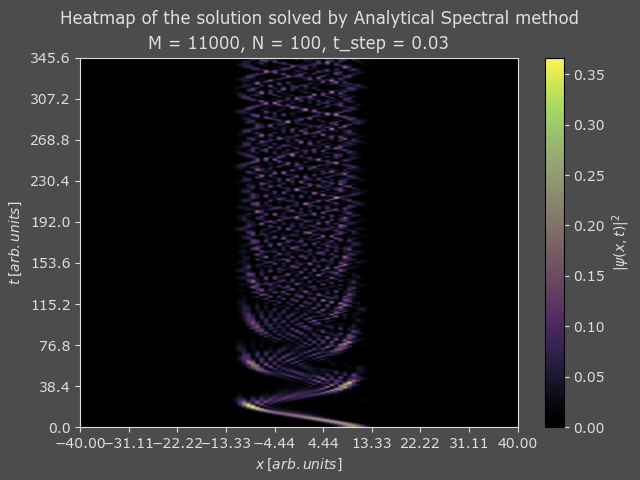
\includegraphics[width=\textwidth]{./images/case1_N100.png}
    \caption{Rešitev pri $N=100$,$M=11000$.}
    \label{fig:harmonic_oscillator_N100}
\end{figure}

Na Sliki \ref{fig:harmonic_oscillator_N100} vidimo, da kljub temu, da je časovna mreža zelo fino diskretizirana,
 se rešitev še vedno razleti.
Zanimivo je, da se razleti na drugačen način kot pri originalnih parametrih. Vzorec je drugačen. Nisem 
pa prepričan zakaj pride do tega. 

\begin{figure}[p]
    \centering
    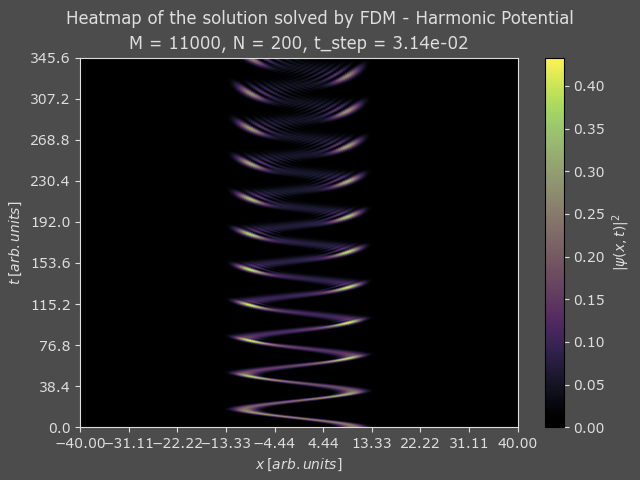
\includegraphics[width=\textwidth]{./images/case1_N200.png}
    \caption{Rešitev pri $N=200$,$M=11000$.}
    \label{fig:harmonic_oscillator_N200}
\end{figure}

Slika \ref{fig:harmonic_oscillator_N200} prikazuje našo spodnjo mejo za smiselen $N$. 
Rešitev se malo razleze, ampak pride skozi 10 nihajev v relativno celem stanju, tako da se zdi zadostno.

\begin{figure}[p]
    \centering
    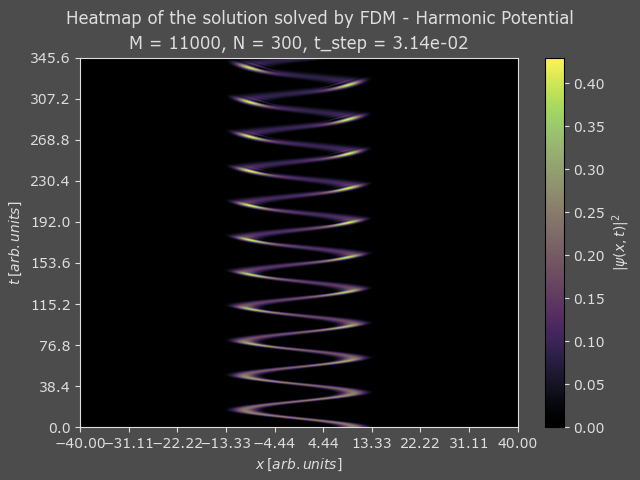
\includegraphics[width=\textwidth]{./images/case1_N300.png}
    \caption{Rešitev pri $N=300$,$M=11000$.}
    \label{fig:harmonic_oscillator_N300}
\end{figure}

Na Sliki \ref{fig:harmonic_oscillator_N300} je rešitev pri originalnih parametrih, samo z bolj fino časovno mrežo.
Rešitev tu je zelo lepa. Vedno manj je deformacij. 

\begin{figure}[p]
    \centering
    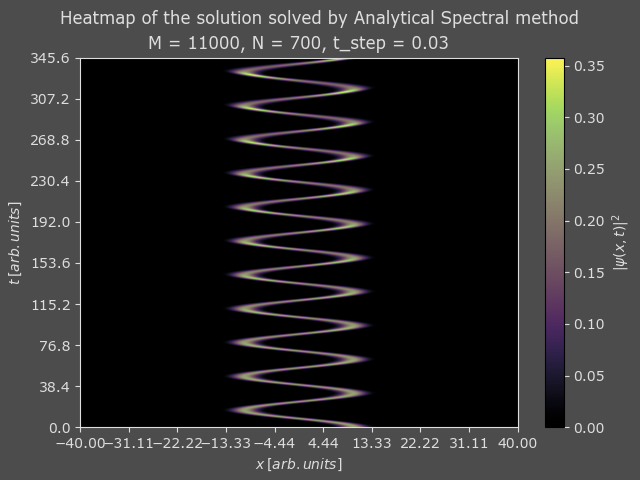
\includegraphics[width=\textwidth]{./images/case1_N700.png}
    \caption{Rešitev pri $N=700$,$M=11000$.}
\end{figure}

Načeloma imam tudi sliko še za $N=500$ ampak je že precej podobna tej, tako da sem jo izpustil.
Tole je pa rešitev pri $N=700$. Pride skozi 10 nihajev brez, da bi bilo opaziti kake res hude deformacije.
Za primerjavo pa seveda še analitična rešitev na Sliki \ref{fig:harmonic_oscillator_analytic}.

\begin{figure}[p]
    \centering
    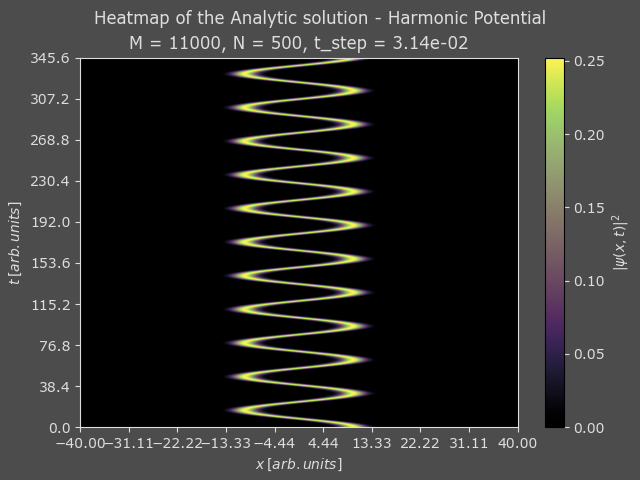
\includegraphics[width=\textwidth]{./images/case1_analytic.png}
    \caption{Analitična rešitev.}
    \label{fig:harmonic_oscillator_analytic}
\end{figure}

Lahko si na hitro pogledamo še odstopanje med analitično in numerično rešitvijo na Sliki \ref{fig:harmonic_oscillator_error}.

\begin{figure}[p]
    \centering
    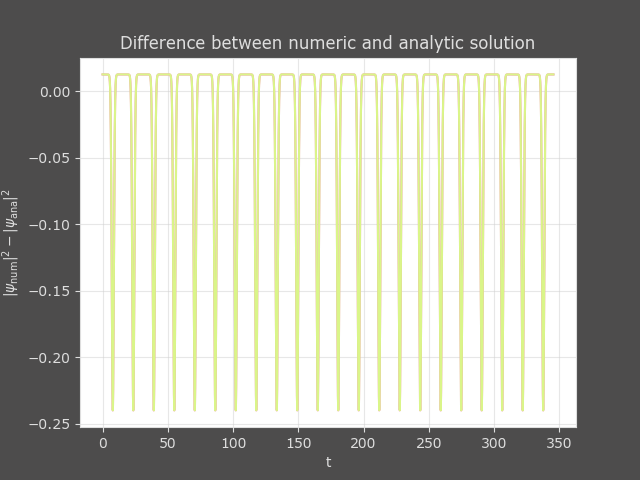
\includegraphics[width=\textwidth]{./images/delta_numeric_analytic_N700.png}
    \caption{Odstopanje med analitično in numerično rešitvijo.}
    \label{fig:harmonic_oscillator_error}
\end{figure}

V tem primeru je bila risana rešitev z $N=700$, v primerjavi z analitično. Brez absolutne vrednosti
čez, kar nam da nekakšen residum. V bistvu delam neke sorte odstopanje med krajevnimi povprečji rešitev. 
V praktičnem smislu se ta vzorec vidi kot zaostajanja numerične rešitve za analitično, kjer jo potem na 
robu potenciala za kratek čas prehiti in začne spet zaostajati. To se vidi fantastično na animaciji, ki jih
naj bi bilo v repozitoriju oz. upam, da se bom spomnil pripeti tudi v mail. \\

\subsection{Drugi primer - gaussov paket}
Za drugi primer sem uporabil začetno stanje (\ref{zacetno_stanje2}).
Začetno stanje sem diskretiziral z mrežo z $N=500$ točkami. Med pisanjem poročila za to nalogo
sem ugotovil, da je bila podana zveza za $\Delta t$, ki sem jo jaz spregledal. Delajmo se, da je bilo to
v resnici le priporočilo. Sklicujem se na creative freedom naloge. Podobno kot pri prvem primeru, sem tudi
tu časovno mrežo razširil na $M=11000$ točk. Tu ni drugega razloga za točno to številko, kot to, da sem 
elemente kopiral iz prvega primera. \\

Rešitev, ki jo dobimo za $N=500$ je na Sliki \ref{fig:gaussian_org}.

\begin{figure}[p]
    \centering
    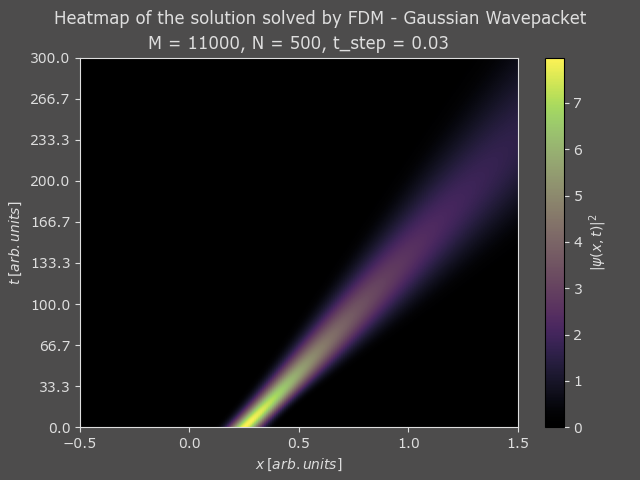
\includegraphics[width=\textwidth]{./images/case2_N500_expanded.png}
    \caption{Rešitev pri $N=500$, $M=11000$.}
    \label{fig:gaussian_org}
\end{figure}

\begin{figure}[p]
    \centering
    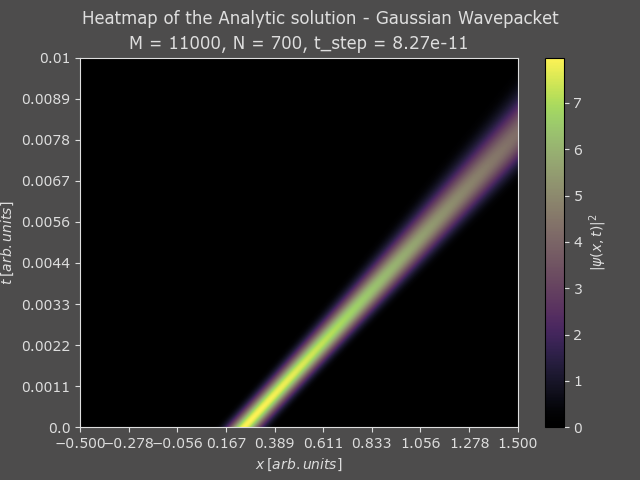
\includegraphics[width=\textwidth]{./images/case2_analytic.png}
    \caption{Analitična rešitev.}
    \label{fig:gaussian_analytic}
\end{figure}

V primerjavi z analitično rešitvijo na Sliki \ref{fig:gaussian_analytic} se zdi, da je rešitev
še kar dogledna. Proti koncu je res že kar šibka, ampak to bi se dalo hitro popraviti z spremembo
parametrov. To se sicer pokaže prvi znak neke napake v moji implementaciji. V nekem srednjem času
je nisem uspel najti, torej je currently "ignored". Čeprav naj bi predstavljaja isto reč je 
časovna skala pri analitični rešitvi čisto drugačna kot pri numerični. Najbolj verjetno je, da sem
se kje zmotil pri prepisu enačb. In to je tudi razlog, da sem se odločil, da ne bom kazal grafa
razlike med analitično in numerično rešitvijo, ker nima smisla. \\

Čudnosti se ne končajo tu sicer. Pravzaprav, ravno zaradi lack of time, sem mogoče nekoliko goljufal
z rešitvijo. Namreč moj razred \texttt{FDMSolver} v tem primeru deloval čudno na robovih krajevne mreže.
To mislim v tem smislu, da se je valovni paket na robu odbil in potem začel interferirati sam s seboj.
Tudi temu sem namenil debugging session, a nisem uspel najti vzroka. So pa grafi arguably 10x bolj
kul in zanimivi kot če bi samo gledali valovni paket, v praznem prostoru. With that being said,
se mi zdi, da je zdaj čas za še eno galerijo.\\

\subsubsection{Komentarji k galeriji}

\begin{figure}[p]
    \centering
    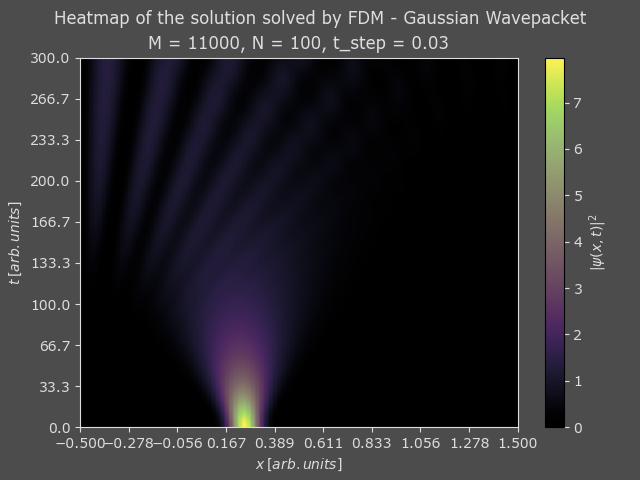
\includegraphics[width=\textwidth]{./images/case2_N100.png}
    \caption{Rešitev pri $N=100$, $M=11000$.}
    \label{fig:gaussian_N100}
\end{figure}

V primeru rešitve za $N=100$ na Sliki \ref{fig:gaussian_N100} rešitev praktično nič ne naredi 
preden se ne raztopi in razpade. Not very interesting. Ampak je pa zanimivo, da je spet $N=200$
spodnja meja za smiselno rešitev, kot nam kaže Slika \ref{fig:gaussian_N200}.

\begin{figure}[p]
    \centering
    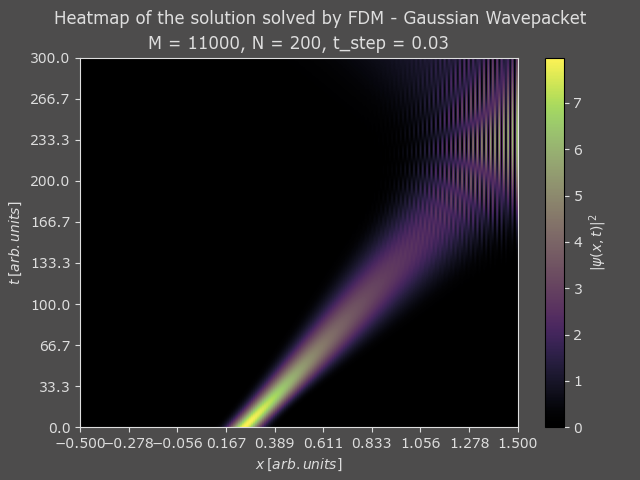
\includegraphics[width=\textwidth]{./images/case2_N200.png}
    \caption{Rešitev pri $N=200$, $M=11000$.}
    \label{fig:gaussian_N200}
\end{figure}

Na Sliki \ref{fig:gaussian_N200} se precej dobro vidi tudi ta čudnost, ki sem jo omenil. 
Valovni paket se odbije od roba in potem začne interferirati sam s seboj. To se še boljše vidi na tej 
Sliki \ref{fig:gaussian_N400}, ki jo imam. Embarraingly enough
se ne spomnem več pogojev nastanka te slike, čeprav je nekaj parametrov zapisanih na njej. V splošnem
naj bi prikazovala isti proces le pri $N=400$ in na daljši časovni skali (razen, da je zaradi nekega 
razloga časovna skala tu manjša). ((Ima to veze z analitično rešitvijo? Me tepe ne poslušanje navodil?))
V glavnem, se odbije in praktično izgine, ker je tako razlezen. Potem pa se začne pojavljati na drugi
stran, kjer se spet tako kot prej odbije ipd.

\begin{figure}[p]
    \centering
    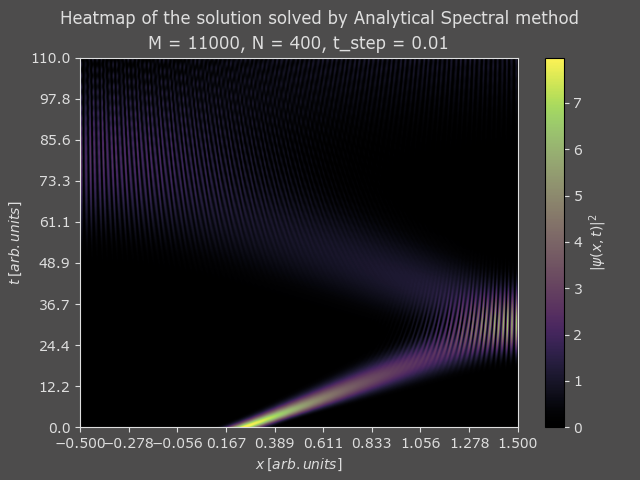
\includegraphics[width=\textwidth]{./images/case2_N400.png}
    \caption{Unknown rešitev pri $N=400$, $M=11000$.}
    \label{fig:gaussian_N400}
\end{figure}

Meni so te interferenčne proge in vzorci res všeč. Tako da obvezno še $N=700$ in potem se ustavim. 

\begin{figure}[p]
    \centering
    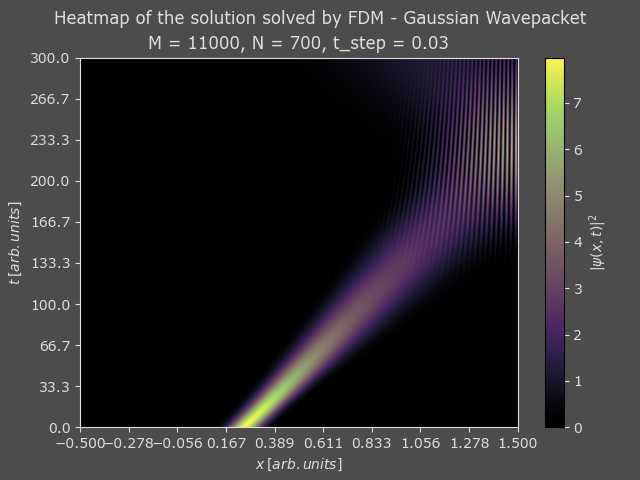
\includegraphics[width=\textwidth]{./images/case2_N700.png}
    \caption{Rešitev pri $N=700$, $M=11000$.}
    \label{fig:gaussian_N700}
\end{figure}

Tu na Sliki \ref{fig:gaussian_N700} se mi zdi, da se fenomenalno vidi vzorec. 
Vztrajal sem, da rabimo ta graf zato, da lahko kot pri  prvi nalogi narišemo še primerjalni plot 
med $N=700$ in $N=200$ rešitvijo. Spet se izkaže, da je razlika izredno majhna, čeprav je nekoliko 
večja kot pri prejšnji nalogi.

\begin{figure}[p]
    \centering
    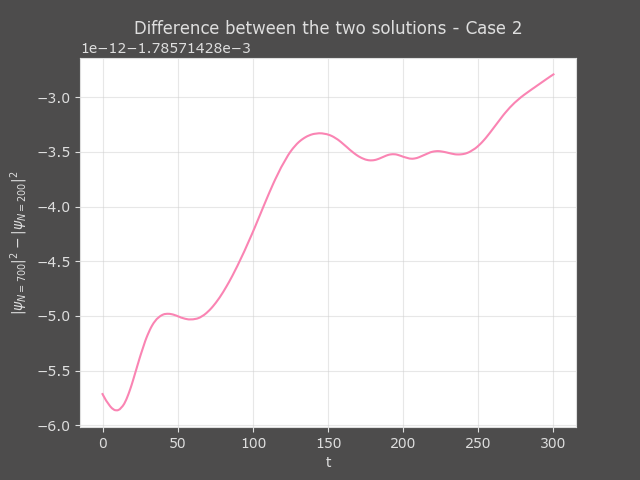
\includegraphics[width=\textwidth]{./images/delta_case2.png}
    \caption{Razlika med rešitvama z $N=700$ in $N=200$}
\end{figure}

\section{Komentarji in izboljšave}
\st{Želim si, da bi imel čas se igrati z LaTeX-om, da bi lahko slike lepše vstavil v poročilo, ker tole 
je obupno, amapak it is what it is.} Do neke mere se mi zdi, da sem malo uredil, s tem, da sem premaknil slike 
na svoje strani in ustvaril kvazi-galerije. Veliko želj sem imel še za to nalogo, ampak se mi tako mudi z vsem,
da res ne gre. Žal mi je, da nisem imel časa narediti več. As of writing naj bi imel ustni izpit čez okoli
dva dneva in nisem še niti začel z učenjem. Tako da se mi zdi, da je to to. Upam, da sem ostale stvari
ustrezno sproti pokomentiral in da je bilo branje prijetno. Poročilo sem napisal v res zelo sproščenem
stilu.

\begin{quotation}
    \centering
    \textit{The traditional funny has been canceled until further notice.}
\end{quotation}


%\newpage
%\bibliographystyle{unsrt}
%\bibliography{sources}
\end{document}
